\documentclass{standalone}
\usepackage{tikz}
\usepackage{ctex,siunitx}
\usepackage{tkz-euclide}
\usepackage{amsmath}
\usetikzlibrary{patterns, calc}
\usetikzlibrary {decorations.pathmorphing, decorations.pathreplacing, decorations.shapes,}
\begin{document}
\small
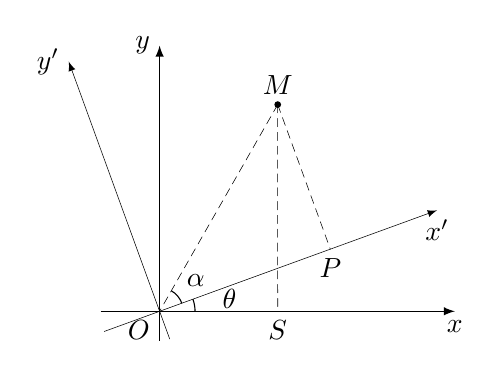
\begin{tikzpicture}[>=latex,scale=0.75]
  \draw[thin,->](-1,0)--(5,0)node[below]{$x$};
  \draw[thin,->](0,-0.5)--(0,4.5)node[left]{$y$};
  \tkzDefPoints{0/0/O,2/3.5/M,1/0/x}
  \tkzDefPointBy[rotation=center O angle 20](x)\tkzGetPoint{x'}
  \tkzDefPointBy[projection=onto O--x](M)\tkzGetPoint{S}
  \tkzDefPointBy[projection=onto O--x'](M)\tkzGetPoint{P}
  \tkzDrawSegments[densely dashed](M,S M,P M,O)
  \tkzMarkAngle[size=0.6](x,O,x')
  \tkzLabelAngle[pos=1.2](x,O,x'){$\theta$}
  \tkzMarkAngle[size=0.4](x',O,M)
  \tkzLabelAngle[pos=0.8](x',O,M){$\alpha$}
  \tkzDrawPoints[fill=black](M)
  \tkzLabelPoints[below left](O)
  \tkzLabelPoints[above](M)
  \tkzLabelPoints[below](S,P)
  \begin{scope}[rotate=20]
    \draw[very thin,->](-1,0)--(5,0)node[below]{$x'$};
    \draw[very thin,->](0,-0.5)--(0,4.5)node[left]{$y'$};
  \end{scope}
\end{tikzpicture}
\end{document}